\documentclass[a4paper,english,12pt,bibliography=totoc]{scrreprt}

\usepackage[T1]{fontenc} %immer
\usepackage[utf8]{inputenc} %am
\usepackage{babel} %Anfang

\usepackage{enumitem} %Aufzählungen verändern

%Gleichungen verwenden
\usepackage{newtxtext}
\usepackage{amsmath}
\usepackage{amssymb}
\usepackage{mathptmx}
%\usepackage{txfonts}

\usepackage{listings}% code blocks
\usepackage[most]{tcolorbox}

%Querverweise
\usepackage{varioref} %immer
\usepackage{hyperref} %in dieser
\usepackage{cleveref} %Reihenfolge

\usepackage{booktabs} %schönere Tabellen
\usepackage{siunitx} %SI-Einheiten
\usepackage{tabularx} %Tabellen mit flexiblen Spalten	

\usepackage{graphicx} %Grafiken verwenden

\usepackage{lipsum} %Blindtext
\usepackage{subcaption}
\usepackage{afterpage}
\usepackage[headsepline]{scrlayer-scrpage} %Paket für Kopfzeilen
\usepackage{afterpage}
\usepackage{float}
\automark[subsection]{section}

\pagestyle{scrheadings}
\ihead{} % oben links
\chead{\leftmark} % oben Mitte
\ohead{} % oben rechts
\cfoot{\pagemark} % unten Mitte
\automark[section]{section} % Modified line

% Zu volle hboxen korrigieren
\tolerance 1414
\hbadness 1414
\emergencystretch 1.5em
\hfuzz 0.3pt
\widowpenalty=10000
\vfuzz \hfuzz
\raggedbottom

%Informationen über das Dokument
\date{\today}


\begin{document}


\begin{titlepage}
	\centering
	
\includegraphics[width=0.8\textwidth]{logo_uulm_sw}
	
	\vspace{1cm}
	\LARGE Compulsory Module for Master Programs
	\Huge \textbf{Biophysics Lab Course}
	
	\vspace{1cm}
	\Large Experiment:

	\Huge \textbf{Atomic Force Microscope}
	
	\vspace{15mm}
	\Large Performed on 29.11.2023
	
	\vspace{5mm}
	\LARGE Group Number 8
	
	\vspace{1cm}
	\Large
	\begin{tabular}{rcl}
	\textbf{Haiyang Zhang} & and & \textbf{Nicolae Turcan}\\
	\href{mailto:student.1@uni-ulm.de}{haiyang.zhang@uni-ulm.de} & & \href{mailto:student.2@uni-ulm.de}{nicolae.turcan@uni-ulm.de}
	\end{tabular}
	
	\vspace{7mm}
	Supervisor: Dr. Carolin Grandy 
	
	\vfill
	\begin{tabular}{p{50mm}@{\hspace{5cm}}p{50mm}}
	\centering \underline{} & \centering \underline{} 
	%\hrulefill & \hrulefill 
	\end{tabular}
	
	\vspace{5mm}
	\normalsize \raggedright
	We hereby confirm that we have elaborated the present work independently and have detailed knowledge of the entire contents.
\end{titlepage}

\tableofcontents

\chapter{Abstract}
\label{cha:abstract}

The Atomic Force Microscope (AFM) is a pivotal tool in biophysical research, offering nanoscale insights into the mechanical properties of biological surfaces. [1] This study employs AFM to investigate fixed mouse fibroblasts (NIH/3T3 ATCC cell line) to understand the impact of cytochalasin D treatment on cell stiffness. The experiment involves force-distance measurements using the JPK NW3 AFM in force-volume mode. Cytochalasin D, a fungal toxin disrupting actin polymerization, serves as the treatment. The objective is to determine if cytochalasin D induces a reduction in cell stiffness, shedding light on cytoskeletal dynamics and cellular responses. The analysis employs the Hertz fit model to calculate Young's modulus. Results are presented through visual representations of Young's modulus, offering immediate insights into material behavior. Morphological differences between treated and untreated cells are explored, emphasizing the connection between cell shape and function. 
%The discussion touches upon scale normalization, striping artifacts, and background consistency. While quantitative analysis is limited, qualitative observations highlight the need for further investigation. This report contributes to the biophysics field by unraveling the intricate interplay between cellular mechanics and external stimuli.


\chapter{Introduction}

\label{cha:intro}

%\textit{}

The Atomic Force Microscope (AFM) sits at the forefront of biophysical research, particularly in its application to probe the nanoscale features and mechanical properties of biological surfaces. A cantilever with a tip scans the sample's surface, providing not only high-resolution imaging but also enabling force spectroscopy. This technique allows us to measure the mechanical properties of living materials, such as cells and tissues, and detect structures with different stiffness levels.\newline
For precise tip movement, a piezo is integral, as changes in voltage induce material expansion due to the piezoelectric effect. This feature enables minimal positioning of the tip. The interaction between the tip and the sample can be described using the Lennard Jones potential, acting as an approximation of forces between two atoms during an approach.\newline
The AFM can operate various distance regimes, we can distinguish between contact and non-contact modes. The former involves repulsive forces at close proximity, while the latter features attractive interatomic forces at a greater distance from the surface. Various AFM measurement modes, including contact, non-contact, tapping, force-volume mode, offer distinct advantages and applications.\newline
As the cantilever's tip approaches the sample, interactions occur, causing bending or deflection. A reflected laser on the cantilever's backside captures these movements. Through precise calibration, the force on the tip is calculated, offering topographical and mechanical information. Utilizing a feedback loop, the tip's movement in relation to the sample produces a comprehensive map of surface topography.\newline
In Force-Volume mode, the cantilever's tip approaches the sample until contact is established and then retracts, measuring the vertical force between the tip and the sample. The resulting force vs. distance curve provides valuable information about local stiffness and adhesion. The slope of the linear part of the curve is associated with the Young’s modulus of the system, offering a means to determine mechanical properties across the sample surface.\newline
\[\textbf{F} = \frac{4}{3}\cdot \frac{\text{E}}{1-v^{2}}\cdot \sqrt{\text{Rd}^{3}}\]

The choice of tip shape is critical, influencing the resolution and suitability for specific measurements. Tetrahedral and pyramidal tips are durable but less suitable for high-resolution imaging. Spike tips or very thin tips, although more fragile and expensive, are ideal for achieving high resolution. Spherical, blunter tips with a larger interaction area are preferable when measuring nanomechanical properties such as Young’s modulus or dealing with Cells.\newline
SPM images, while interpretable, are susceptible to artifacts such as tip convolution. The resolution is inherently tied to the tip's shape, and each data point represents a spatial convolution of the tip and the imaged feature. Common artifacts include tip imaging, particularly prominent in samples with abrupt features.\newline
In the present study, the aim is to investigate the mechanical properties of fixed mouse fibroblasts (NIH/3T3 ATCC cell line) using AFM. The motivation behind this experiment is to understand how cells respond to a treatment with cytochalasin D, a fungal toxin known to interfere with actin polymerization. The final objective is to determine if cytochalasin D treatment results in a reduction of cell stiffness. This investigation has significant implications for understanding the role of the cytoskeleton and how alterations in its dynamics impact the mechanical properties of cells.\newline
The experimental setup involves measuring force-distance curves in force-volume mode on a JPK NW3 AFM. Before the measurement, the cells are fixed with 4 percent formaldehyde, and for one set of measurements, cells are treated with cytochalasin D (\(2\mu \text{M}\)) for 30 minutes before fixation. The Young's modulus is determined by using the Hertz fit model in the lab. This approach provides a comprehensive understanding of the mechanical properties of the cells, aiding in the elucidation of cytoskeletal dynamics and responses to external stimuli.\newline
In the subsequent sections of this report, we delve into the experimental methodology, results, and discussions derived from the AFM analysis of the cell surfaces. Through a detailed examination of the topography and mechanical properties, we aim to contribute to the growing body of knowledge in the field of biophysics, specifically in the context of cellular mechanics and AFM applications.\newline


\chapter{Material and Methods}
\label{cha:exp}

\section{Material}
\label{sec:material}

\begin{table}[h]
\centering
\begin{tabular}{|c|c|}
  \hline
  Material & model \\
  \hline
  Atomic force microscopy (AFM) & JPK NW3 AFM \\
    \hline
  mouse fibroblasts & NIH/3T3 ATCC \\
    \hline
  chemical & 4\% formaldehyde\\
    \hline
  chemical &  cytochalasin D (\(2\mu \text{M}\))\\
  \hline
\end{tabular}
\caption{Materials}
\label{tab:material}
\end{table}

\section{Methods}
\label{sec:methods}
In this experiment, the mouse fibroblasts were treated with 4\% formaldehyde for 10 minutes to fix the cells. Cytochalasin D (\(2\mu \text{M}\)) was used for 30 minutes before fixation. The measurements were conducted using the Force-Volume mode of AFM. Theoretically we would use the spherical tip, but we used the tetrahedron tip instead.
The Young's modulus is determined by using the Hertz fit model in the lab with the JPK program. The analysis and graphs in this report were generated using Julia.

\chapter{Experiment and Analysis}
\label{cha:experimenandanalysis}  

\section{Experiment}
\label{sec:experiment} 
The Experiment was conducted in the following way: \newline
1) A new tip was picked with tweezers and placed onto the glass block and fixed with a lever. \newline 
2) The measuring Block was inserted into the Instrument. \newline 
3) A Calibration of the AFM was performed.\newline
4) Then we  Introduced the Petri Dish with Cultured Cells inside the AFM stage. \newline 
5) The Tip Approached the sample. \newline
6) A table light was lit and placed obliquely to the dish to increase contrast and was used to find a candidate Cell for measurement. \newline 
7) The light and Camera modules were switched off. \newline 
8) We performed a  scan to get the raw data and the graphs.\newline
9) JPK Software proprietary to the Instrument was used to calculate the Young's modulus using the Hertz Fit Module.\newline
10) The Tip was lifted  200 micrometers to avoid damage to the tip. \newline 
11) This process was repeated for all the other measurements.

\section{Statistical Analysis}
\label{sec:statanalysis} 

%\subsection{Raw Data JPK Converted}
%\label{subsec:jpk}

%\subsection{Julia as a Platform for .tsv Analysis}
%\label{subsec:Julia}

\subsection{Mean Median and Standard Deviation}
\label{subsec:mmandsd}
A mean is quantity that has a value which is intermediate to the extreme values of a set of numbers.[2] For discrete data, the arithmetic mean is given by the formula:
\[ \text{Mean} = \frac{\text{Sum of all values}}{\text{Number of values}}\]
or in mathematical expression, for samples \(x_1, x_2, \ldots, x_n\),
\[\bar{x} = \frac{\Sigma^n_{i=1} x_i}{n}\]

According to the discussion at 4.2.2, here we compute the mean Young's modulus of the cell, using the data filtered in Figure 4.2.(a) and 4.2.(b),
%\begin{tcolorbox}[colback=black!80!white, coltext=white]
%\begin{lstlisting}[language=python, basicstyle=\ttfamily\small]
%println(mean(ym_cutoff_cell_untreated))
%println(mean(ym_cutoff_cell_treated))

%59178.865403645825
%59446.74919463088
%\end{lstlisting}
%\end{tcolorbox}

In statistics and probability theory, the median is the value separating the higher half from the lower half of a data sample, a population, or a probability distribution.[3]
%then give the median of our data
%\begin{tcolorbox}[colback=black!80!white, coltext=white]
%\begin{lstlisting}[language=python, basicstyle=\ttfamily\small]
%println(median(ym_cutoff_cell_untreated))
%println(median(ym_cutoff_cell_treated))

%57365.7
%53179.5
%\end{lstlisting}
%\end{tcolorbox}
In statistics, the standard deviation is a measure of the amount of variation or dispersion of a set of values.[4] By definition, for samples \(x_1, x_2, \ldots, x_n\), a standard deviation \(\sigma\) is
\[ \sigma = \sqrt{\frac{\Sigma^n_{i=1}(\Bar{x} - x_i)^{2}}{n-1}}
\]

%\begin{tcolorbox}[colback=black!80!white, coltext=white]
%\begin{lstlisting}[language=python, basicstyle=\ttfamily\small]
%println(std(ym_cutoff_cell_untreated))
%println(std(ym_cutoff_cell_treated))

%22271.27021740767
%31334.339853297723
%\end{lstlisting}
%\end{tcolorbox}

\subsection{T-Test}
\label{subsec:ttest}
A t test is a statistical test that is used to compare the means of two groups. It is often used in hypothesis testing to determine whether a process or treatment actually has an effect on the population of interest, or whether two groups are different from one another.[7] In our case, we use two-sample t test. We have null hypothesis $H_0$,posits that there is no significant difference between the means of the two groups, while the alternative hypothesis $H_1$,suggests a significant difference.
Further more, we calculate \textbf{test statistic}
\[t = \frac{(\Bar{x_1}-\Bar{x_2})}{{s_p}\sqrt{{\frac{1}{n_1}}+\frac{1}{n_2}}}\]
where\(\Bar{x_1} , \Bar{x_2}\) are the mean value of two samples, \(n_1 , n_2\) are sample size.\(s_p\) is the \textbf{pooled variance}
\[s_p = \sqrt{\frac{((n_1 - 1)s_1^2)+((n_2-1)s_2^2)}{n_1+n_2-2}}\]
and \({s_1}^{2}, {s_2}^{2}\) are variance of two samples.
In order to test the hypothesis, we compare the test statistics with the t-value acquired from t-distribution, which is decided by the degree of freedom $dF = n_1+n_2-2$, and significance level $\alpha$. If the test statistics is larger than the t-value, we say that under the significance $\alpha$, the $H_0$ is rejected. Otherwise, we fail to reject the $H_0$. And in our experiment, the above parameters are explained as follows:\\

\textbf{Hypothesis:}\\
- \textbf{Null Hypothesis (H0):} No significant difference in Young's modulus exists between cytochalasin D treated and untreated cells. Treatment has no impact on cell stiffness.\\
- \textbf{Alternative Hypothesis (H1):} Cells treated with cytochalasin D are softer, showing a significant decrease in Young's modulus compared to untreated cells.\\

\textbf{Result Interpretation:}\\
- \textbf{Rejecting H0:} A low p-value (\(<0.05\)) signifies sufficient evidence to conclude that cytochalasin D induced a significant softening effect.\\
- \textbf{Failing to Reject H0:} A high p-value implies insufficient evidence, suggesting no clear softening effect.\\

\textbf{Outcome Insight:}\\
- \textbf{Significant Result (Low p-value):} Confirmed that cytochalasin D treatment led to a notable softening in cells.\\
- \textbf{Non-Significant Result (High p-value):} Indicated that the data didn't convincingly support a significant softening effect; the impact of treatment was inconclusive.\\

Our approach leveraged statistical analysis, particularly the t-test, to discern whether cytochalasin D had a discernible influence on cell stiffness, the Violoinplot and Boxplot give immediate visual interpretability to the results.

\chapter{Results and Discussion}
\label{cha:ResandDisc}


%\section{Results}

%\label{subsec:resultsHC}



%\subsection{Cut-off Values}
\section{Young's modulus of the fibroblasts}
\label{subsec:cutoffval}

% \begin{figure}[h]
%   \centering
%   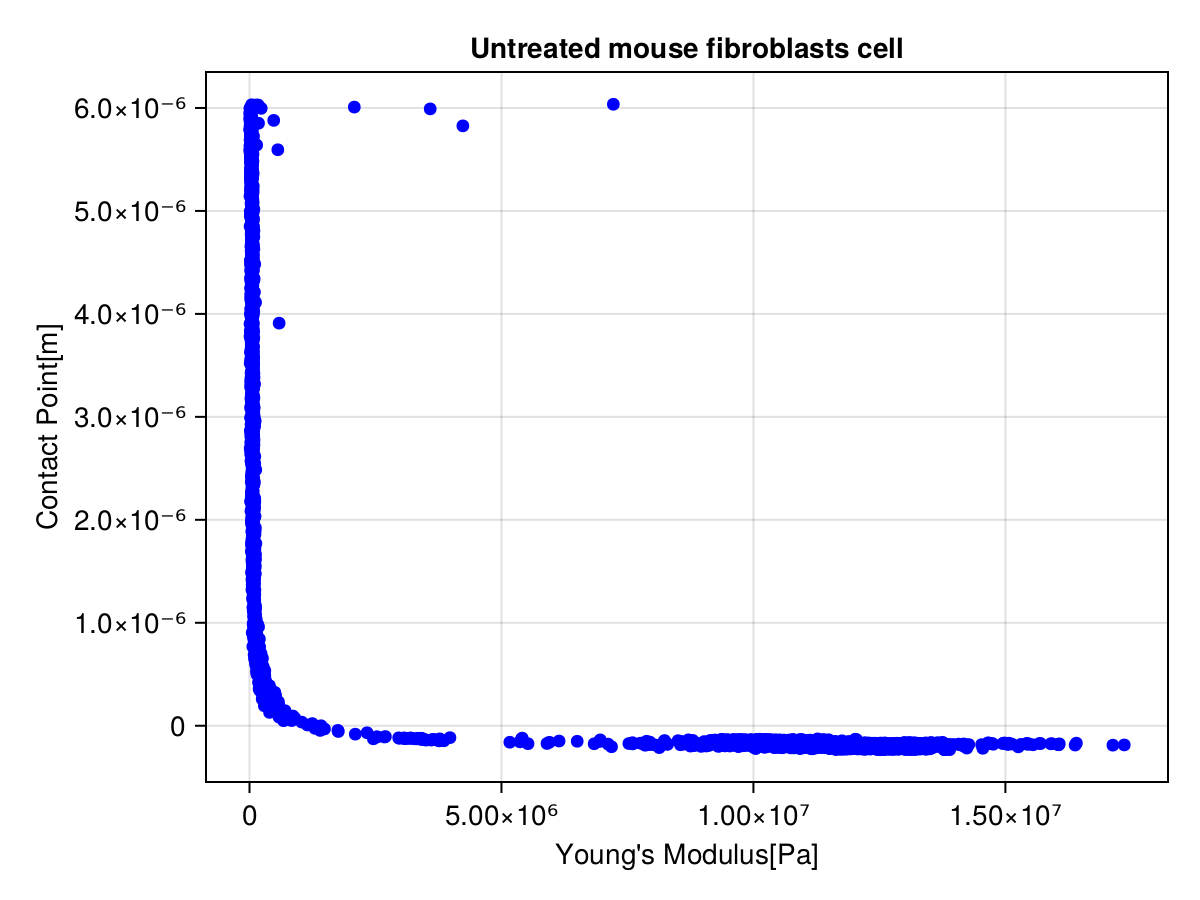
\includegraphics[width=0.8\textwidth]{YM-CP-curve/ym-cp-curve-untreated.png}
%   \caption{Young's modulus and contact point curve of untreated cell}
%   \label{fig:ym_cp_curve_untreated}
% \end{figure}

% \begin{figure}[h]
%   \centering
%   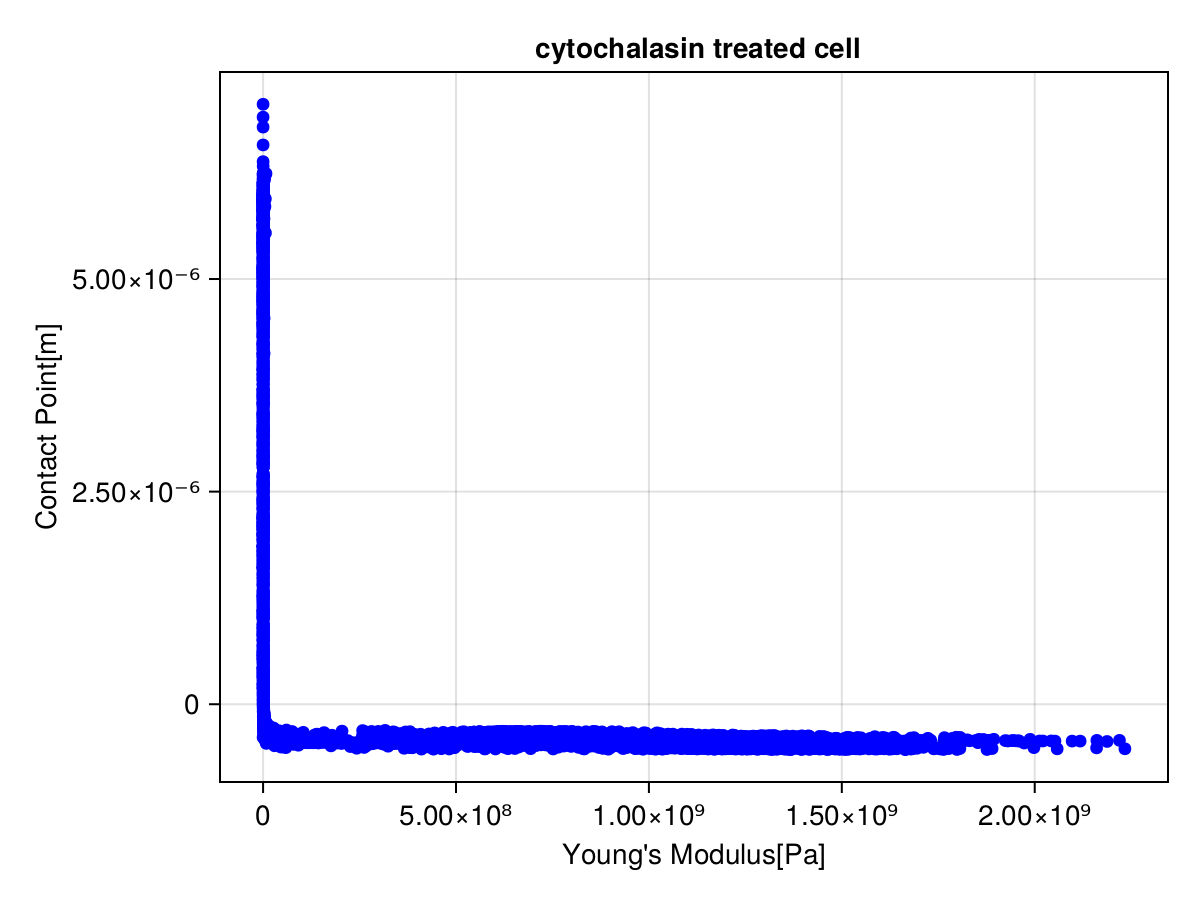
\includegraphics[width=0.8\textwidth]{YM-CP-curve/filtered-ym-cp-curve-untreated.png}
%   \caption{Young's modulus and contact point curve of treated cell}
%   \label{fig:ym_cp_curve_treated}
% \end{figure}

In the experiment, we acquired the contact point through AFM measurement and the young's modulus through JPK program. Figure 5.1.(a) and 5.1.(b) are generated to show the relationship between the young's modulus and the contact point. Observing the figure 5.1, the curve of Young's modulus and contact points, we can conclude that the Young's modulus of the cell should fall along the left vertical line in the figure. This is because the Young's modulus of fibroblasts should be significantly smaller than the background. Besides, we want to filter out the ourliers and the error values, such as the negative contact points. After several attempts, we established the cut-off values for the Young's modulus between 0 to \(2.0 \times 10^{5}\)Pa, while the contact points are restricted between \(1.0 \times 10^{-6}\)m to \(5.0 \times 10^{-6}\)m, as is shown in the restricted area by the red lines in Figure 5.1.\\

The histograms of the Young's modulus of untreated and treated cell are shown in Figure 5.2. The statistical values of the untreated and treated cell are listed in the table 5.1. According to previous research[6], the mean value of Young's modulus of the fixed fibroblasts are around\(5 \times 10^{4}\) Pa, which is at the same scale as the Young's modulus observed in our experiment. T-test was conducted to see the changes of the Young's modulus on the cells treated with cytochalasin, however the result(p-value: 0.8477) says that there are no significant diffenerences on the Young's modulus between treated cell and untreated cell, which contradict to the previous reseach[5],[7].
\begin{table}[h]
\centering
\begin{tabular}{|c|c|c|c|}
  \hline
  Statistical values[Pa] & mean & median & standard deviation\\
  \hline
   untreated fibroblasts & 59178.86 & 57365.7 & 22271.3 \\
    \hline
  treated fibroblasts & 59446.75 & 53179.5 & 31334.3\\
    \hline
\end{tabular}
\caption{Statistical values of the untreated and treated cells}
\label{tab:Statistical_values}
\end{table}

%\begin{tcolorbox}[colback=black!80!white, coltext=white]
%\begin{lstlisting}[language=python, basicstyle=\ttfamily\small]
%#setting the cutoff values
%#cell untreated
%min_ym_untreated = 0.0       
%max_ym_untreated = 2.0e5    #young's modulus
%min_cp_untreated = 1.0e-6
%max_cp_untreated = 5.0e-6   #contact point
%#cell treated
%min_ym_treated = 0.0
%max_ym_treated = 2.0e5
%min_cp_treated = 1.0e-6
%max_cp_treated = 5.0e-6

%\end{lstlisting}
%\end{tcolorbox}


\begin{figure}[H]
    \begin{subfigure}{0.45\textwidth}
        \centering
        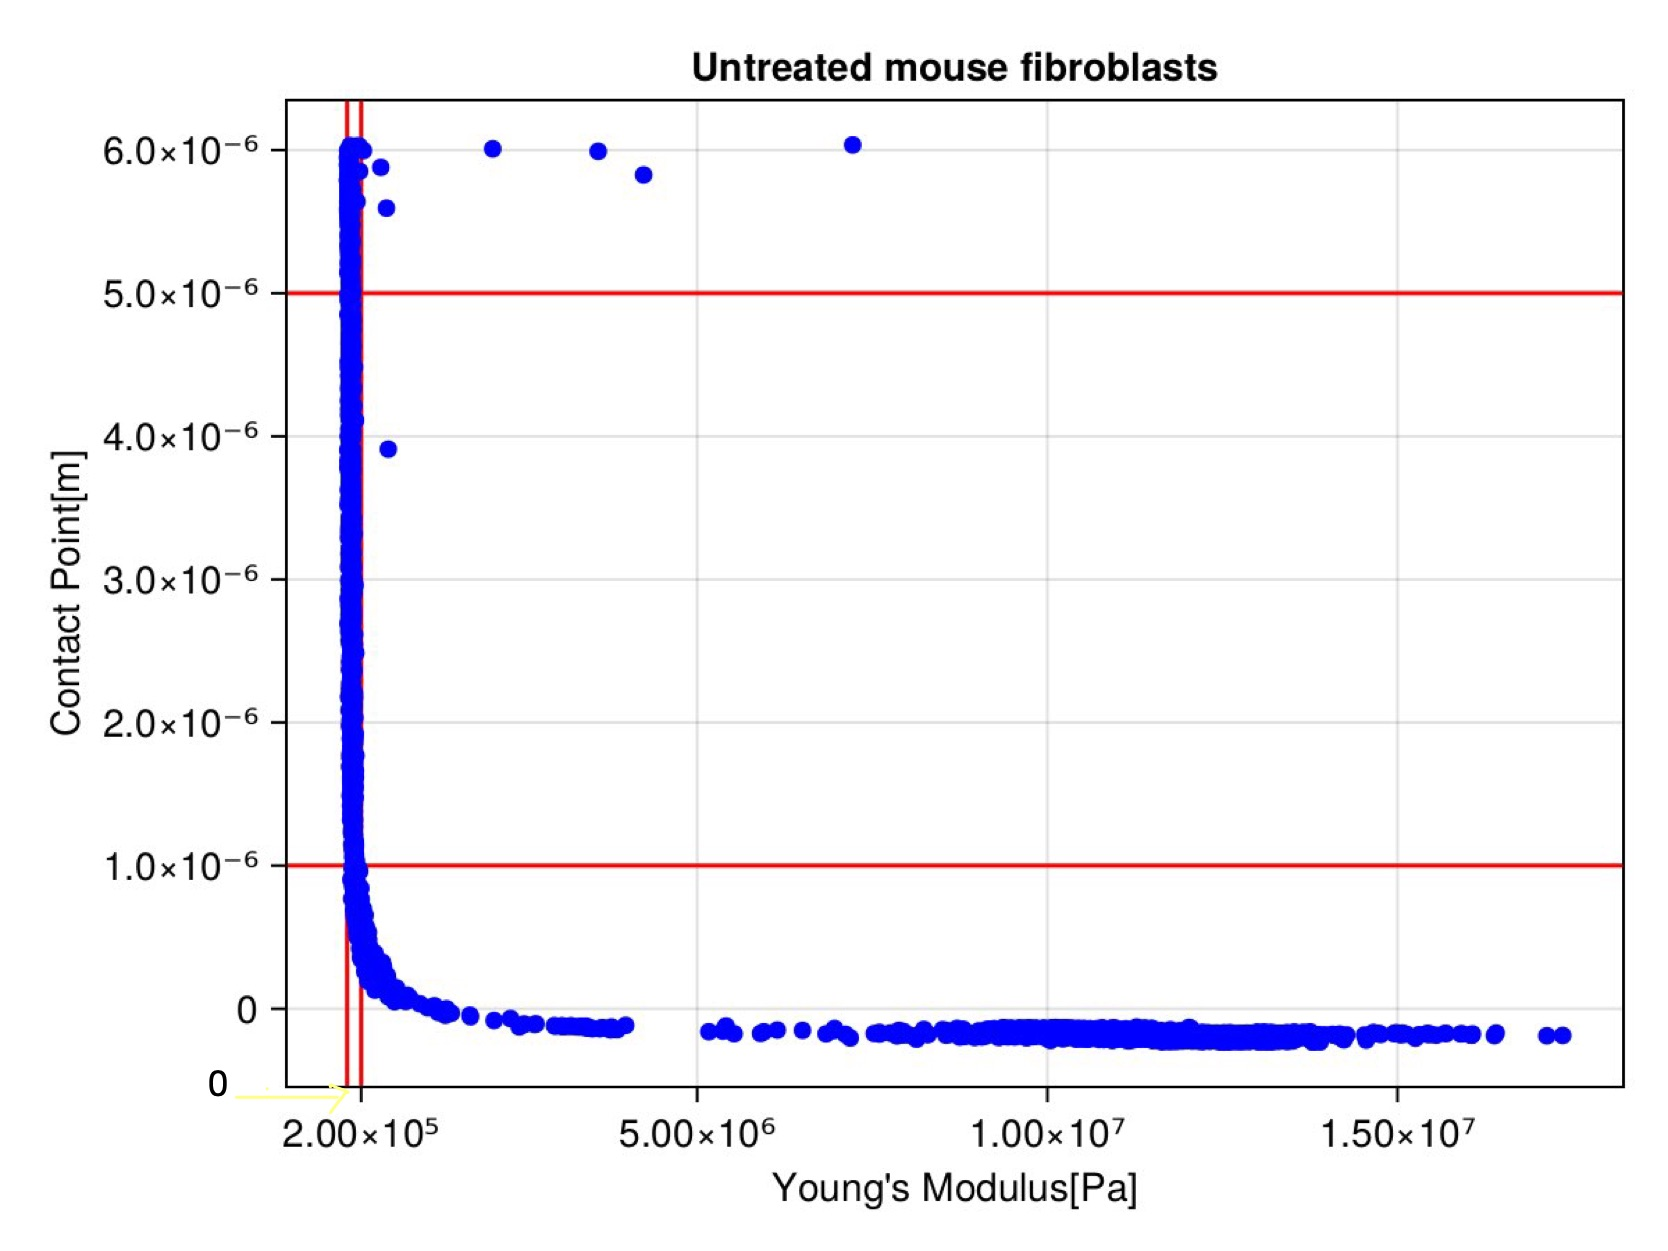
\includegraphics[width=\textwidth]{untreated/ym-cp-curve-untreated-labelled.jpeg}
        \caption{Young's modulus and contact point curve of untreated cell}
        \label{fig:ym_cp_curve_untreated}
    \end{subfigure}
    \begin{subfigure}{0.45\textwidth}
        \centering
        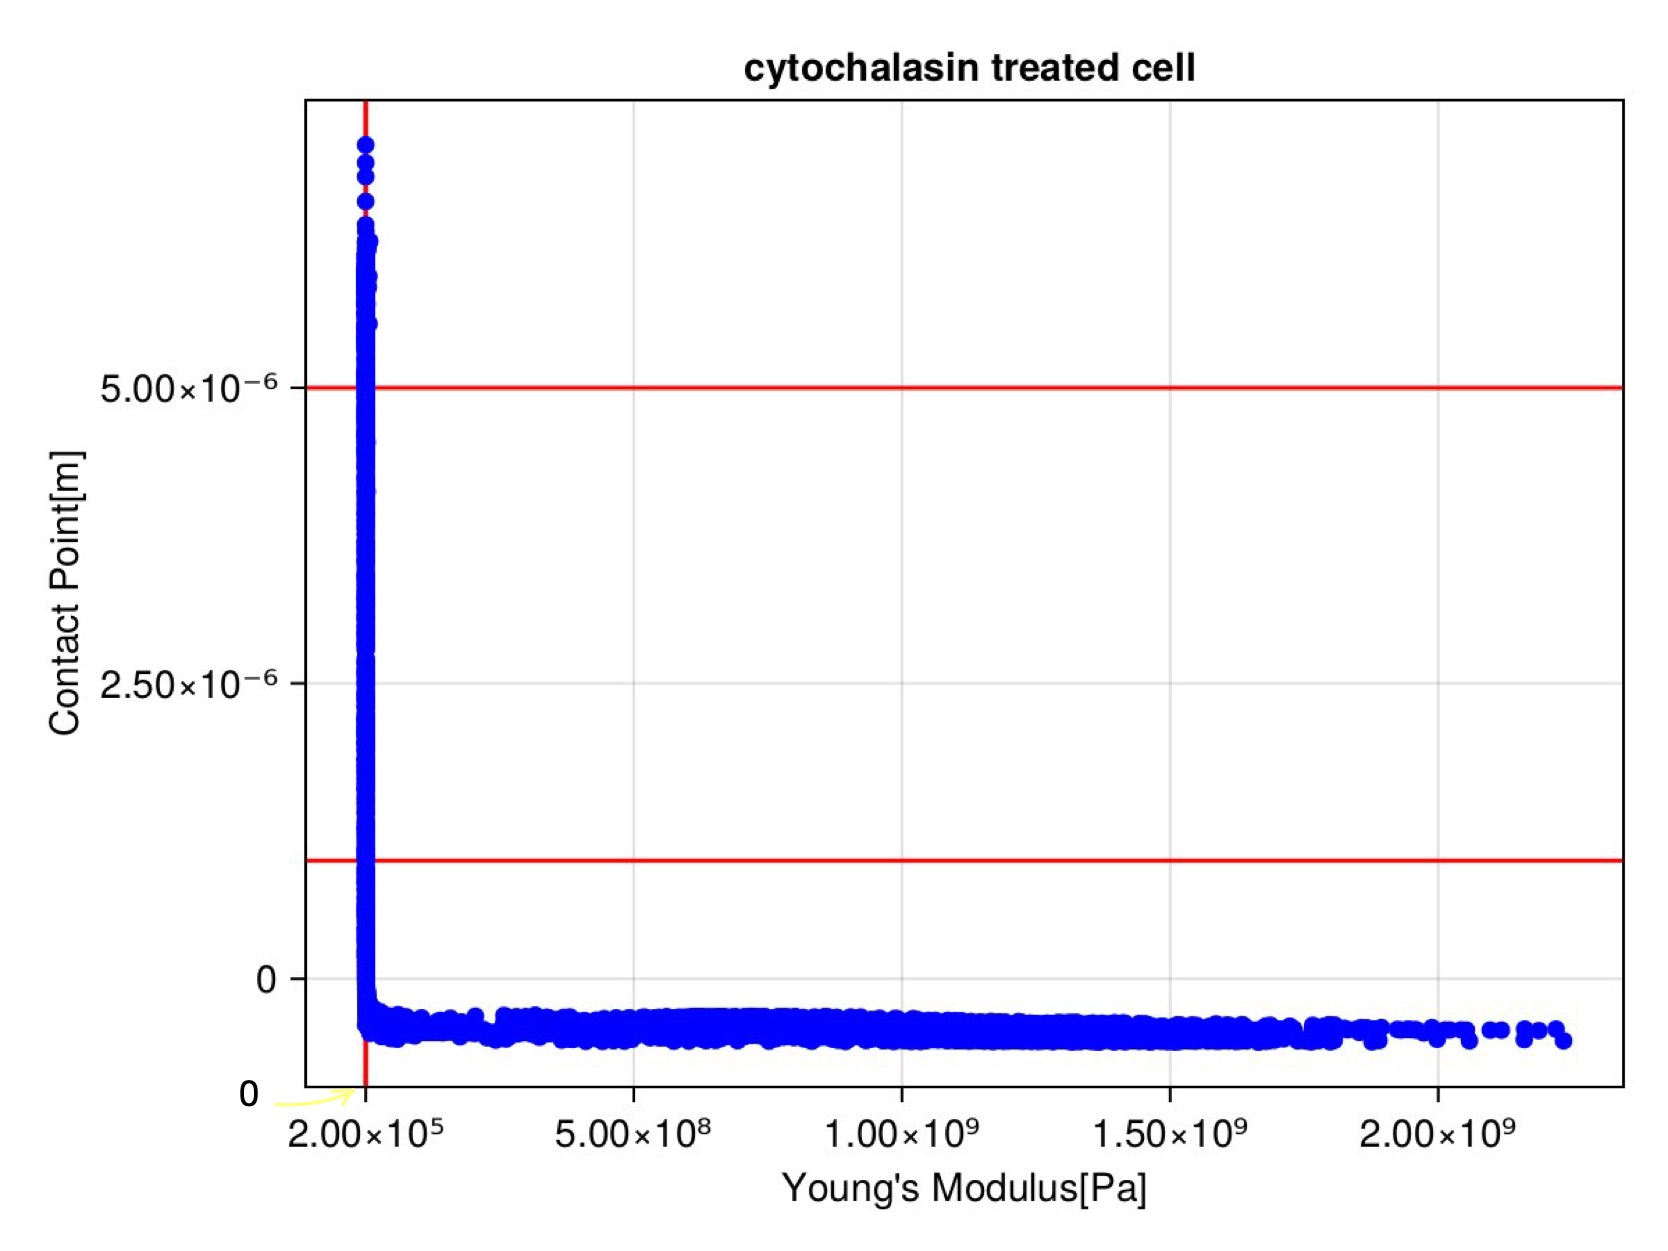
\includegraphics[width=\textwidth]{treated/ym-cp-curve-treated-labelled.jpeg}
        \caption{Young's modulus and contact point curve of treated cell}
        \label{fig:ym_cp_curve_treated}
    \end{subfigure}
    \caption{Young's modulus and contact point}
    \label{fig:ym_cp_curve}
\end{figure}


\begin{figure}[H]
    \begin{subfigure}{0.45\textwidth}
        \centering
        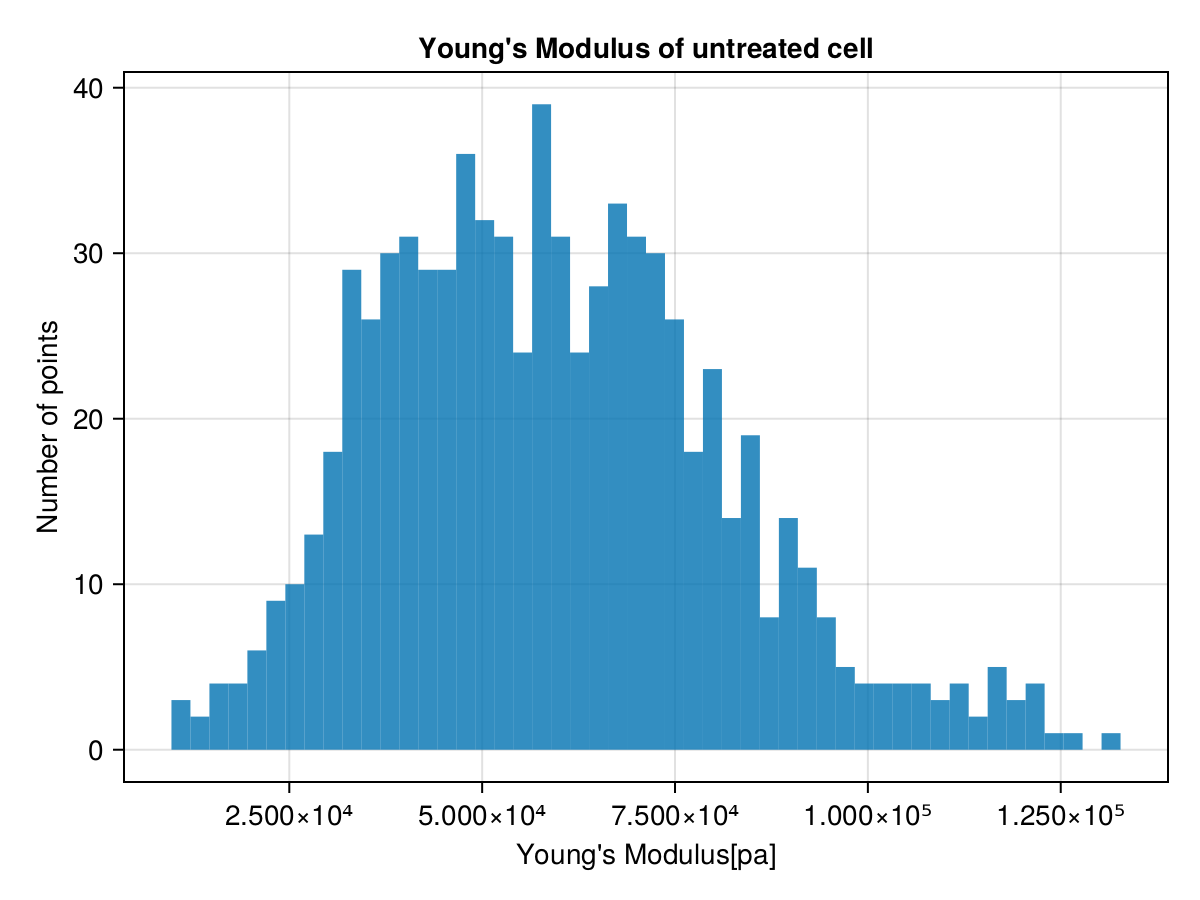
\includegraphics[width=\textwidth]{HistogramsAndViolinplot/histogram_of_untreated.png}
        \caption{Young's modulus of untreated cell}
        \label{fig:ym_cell_untreated}
    \end{subfigure}
    \begin{subfigure}{0.45\textwidth}
        \centering
        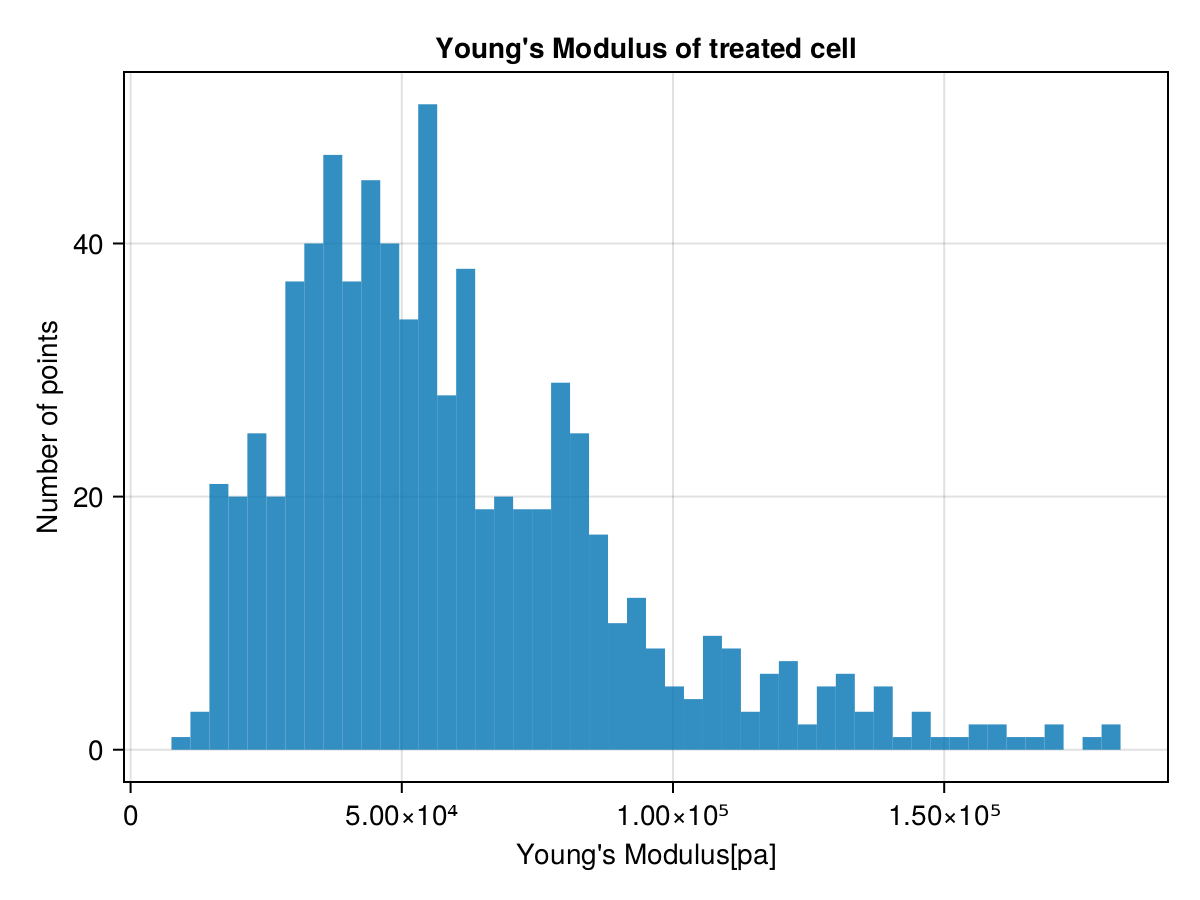
\includegraphics[width=\textwidth]{HistogramsAndViolinplot/histogram_of_treated.png}
        \caption{Young's modulus of treated cell}
        \label{fig:ym_cell_treated}
    \end{subfigure}
    \caption{Young's modulus of cell}
    \label{fig:ym_cell}
\end{figure}




% \begin{figure}[h]
%   \centering
%   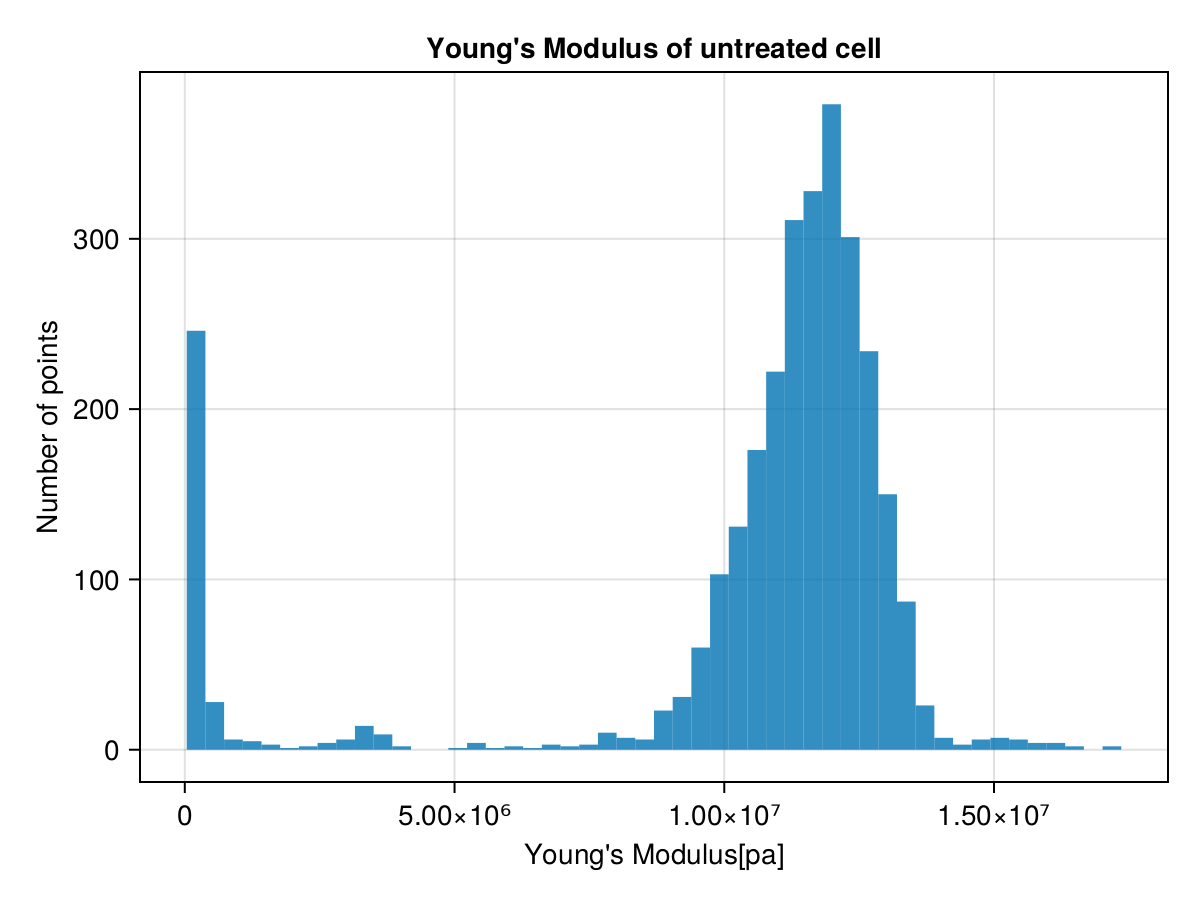
\includegraphics[width=0.8\textwidth]{all datas/histogram_of_untreated.png}
%   \caption{Young's modulus of untreated cells}
%   \label{fig:ym_untreated}
% \end{figure}

% \begin{figure}[h]
%   \centering
%   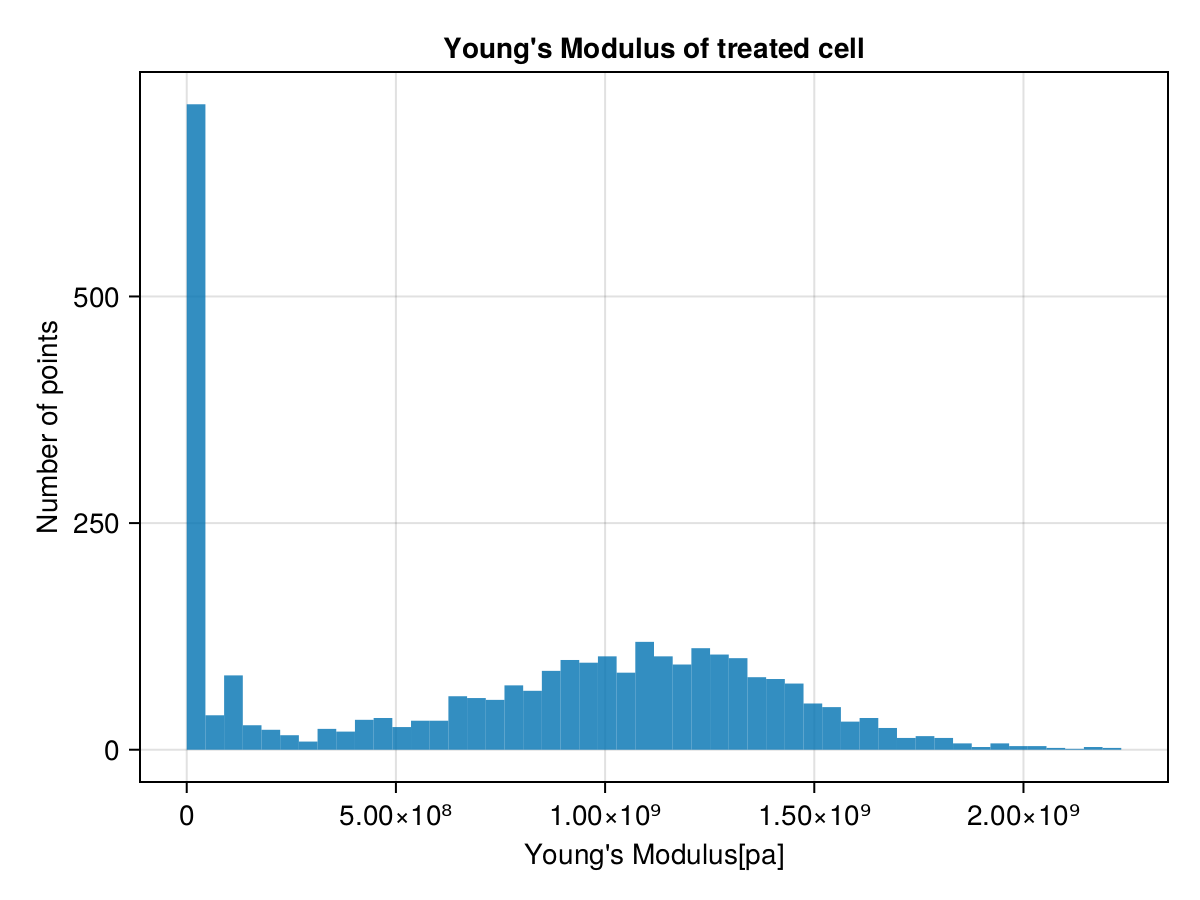
\includegraphics[width=0.8\textwidth]{all datas/histogram_of_treated.png}
%   \caption{Young's modulus of treated cell}
%   \label{fig:ym_treated}
% \end{figure}



%\subsection{Distinction between Cell-like and Surface-like Datapoints}
%\label{subsec:distinctioncellvssurf}

%Figure 4.3.(a) and Figure 4.3.(b) are generated from the filtered Young's modulus of untreated and treated cell. From these graphs, the left peaks in the graphs, at around \(2 \times 10^{5} \) Pa (See Figure 4.5 and 4.6) are the peaks of the cell, while the right peaks are Young's modulus of background. Here, we select the left peaks because, in this context, the background represents the container of the cells, which has a larger Young's modulus than the cells.

%\begin{figure}[H]
%    \begin{subfigure}{0.45\textwidth}
%        \centering
%        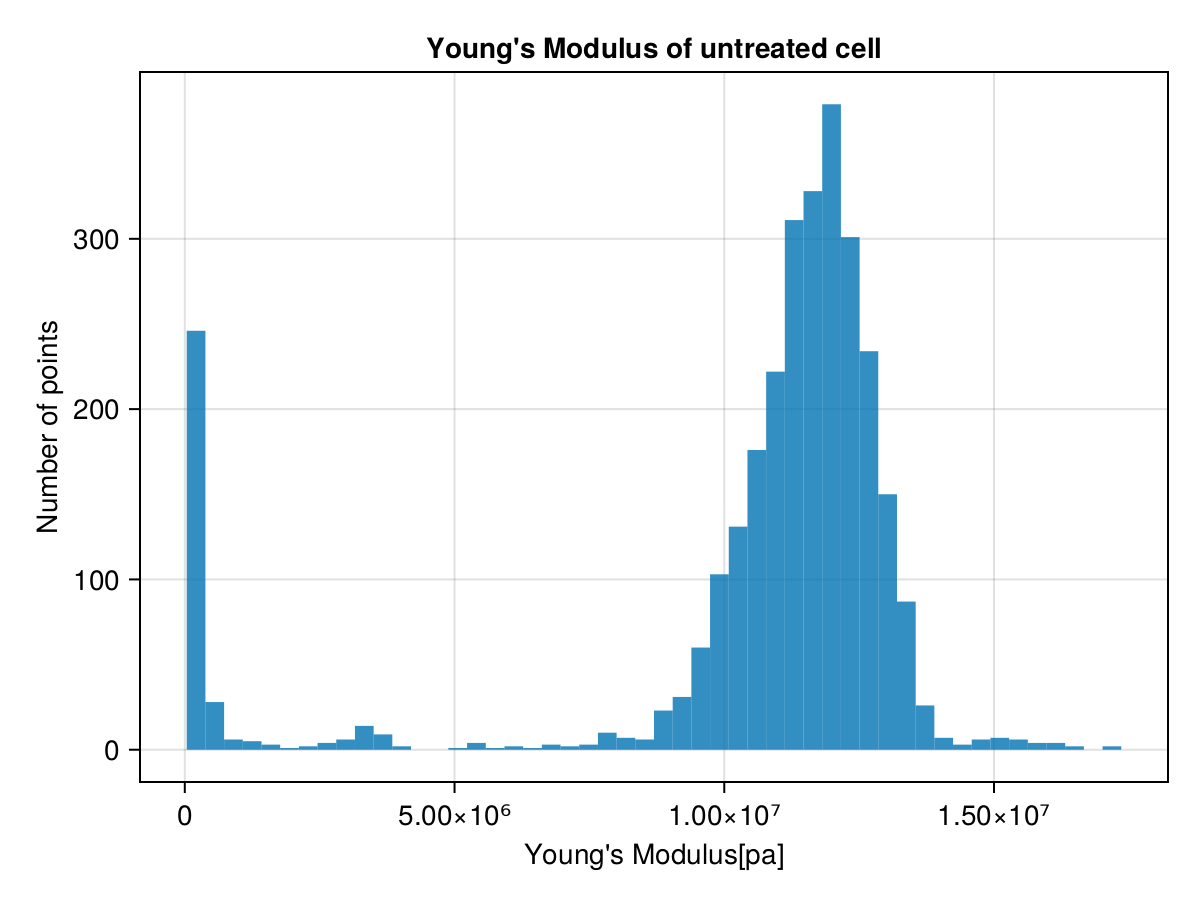
\includegraphics[width=\textwidth]{all datas/histogram_of_untreated.png}
%        \caption{Young's modulus from untreated datas}
%        \label{fig:ym_untreated}
%    \end{subfigure}
%    \begin{subfigure}{0.45\textwidth}
%        \centering
%        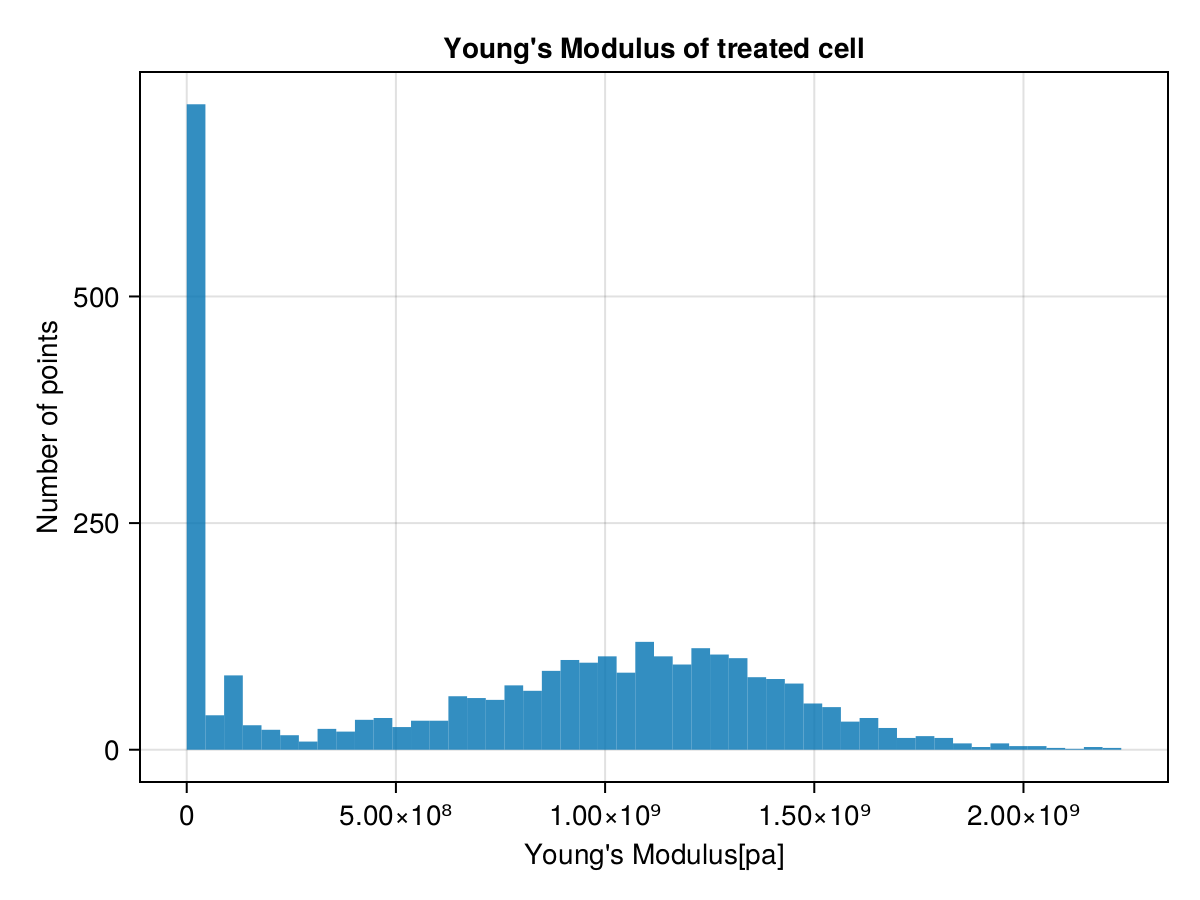
\includegraphics[width=\textwidth]{all datas/histogram_of_treated.png}
%        \caption{Young's modulus from treated datas}
%        \label{fig:ym_treated}
%    \end{subfigure}
%    \caption{Distribution of Young's Modules}
%    \label{fig:main}
%\end{figure}

% \begin{figure}[h]
%   \centering
%   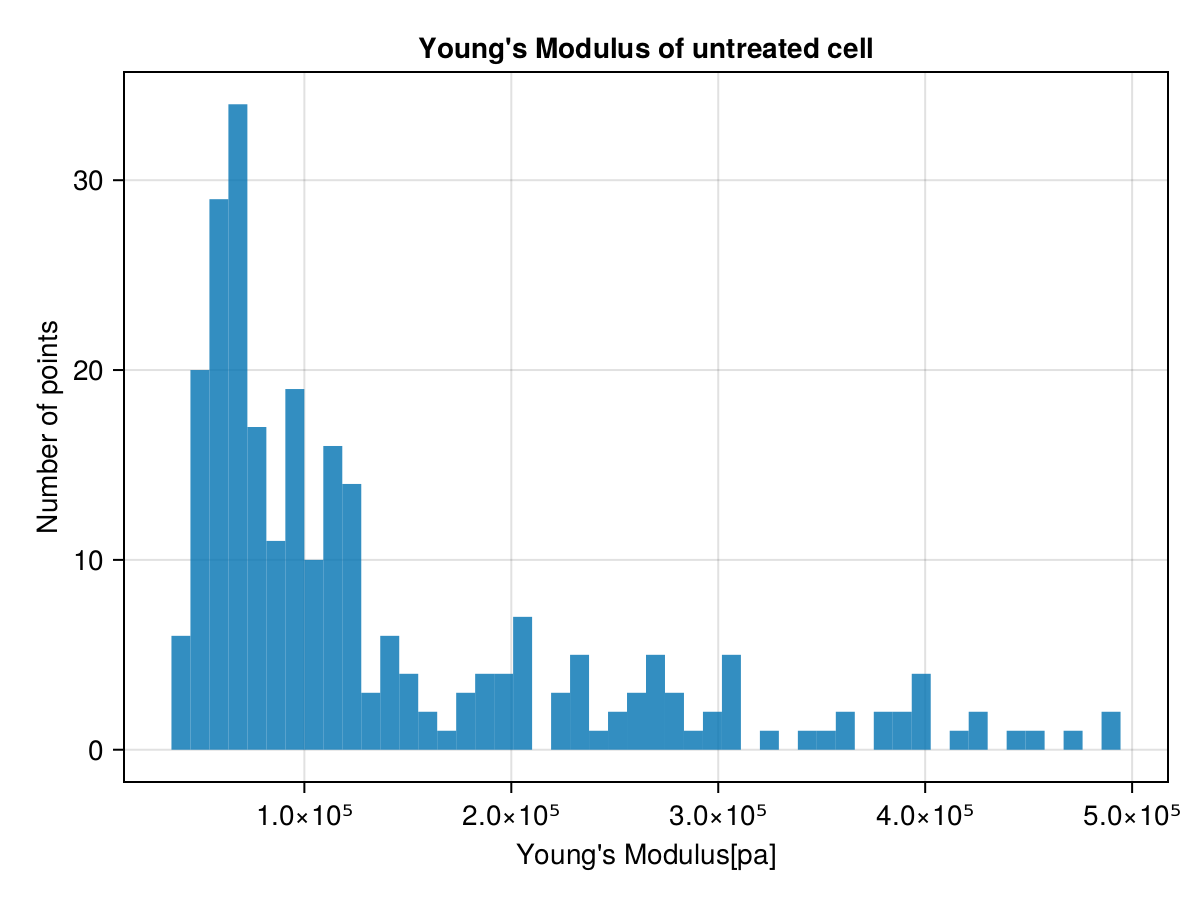
\includegraphics[width=0.8\textwidth]{all datas/ym_cut_histogram_of_untreated.png}
%   \caption{the left side peak of Young's modulus of untreated cells}
%   \label{fig:ym_cut_untreated}
% \end{figure}

% \begin{figure}[h]
%   \centering
%   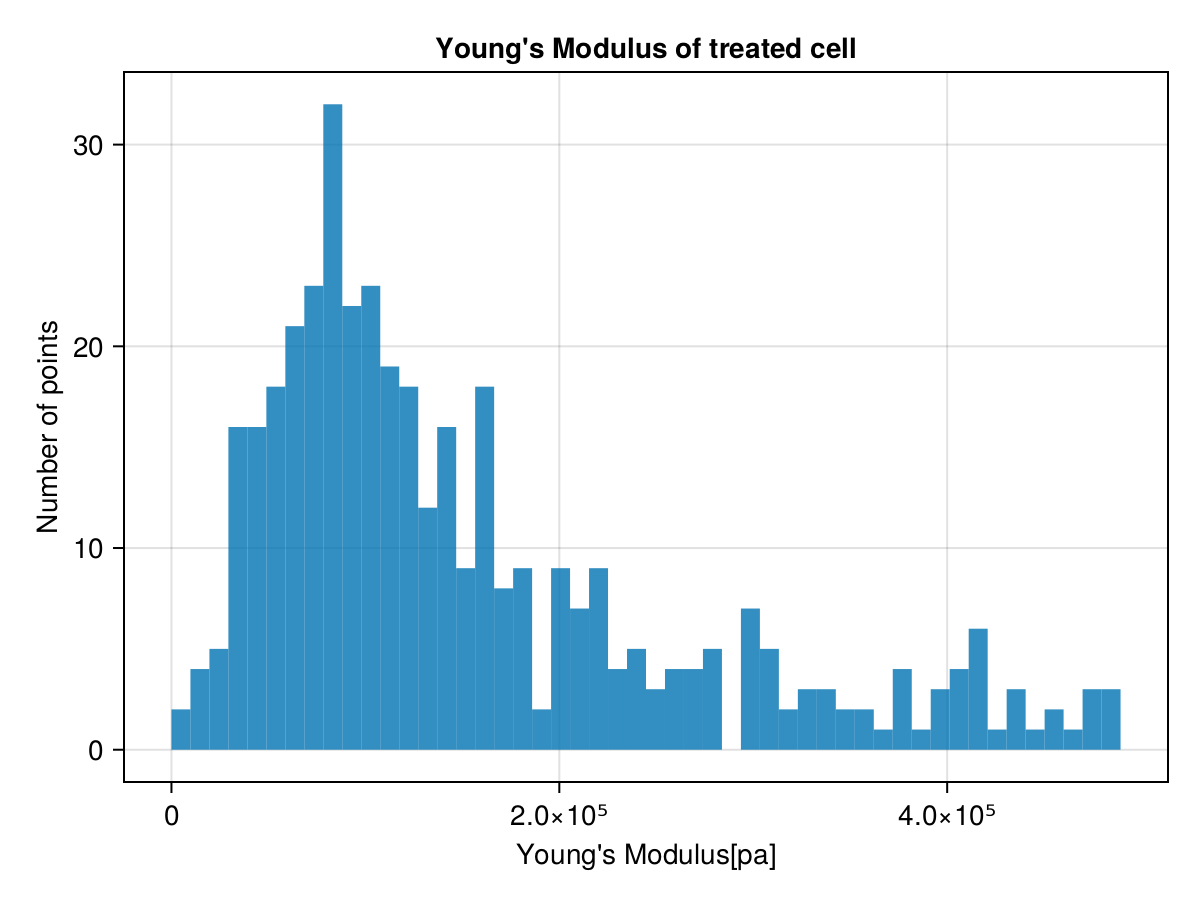
\includegraphics[width=0.8\textwidth]{all datas/ym_cut_histogram_of_treated.png}
%   \caption{the left side peak of Young's modulus of treated cells}
%   \label{fig:ym_cut_treated}
% \end{figure}


A violin plot was used to display the results because it effectively combines aspects of box plots and density estimation, providing a comprehensive visualization of the distribution of data, including its central tendency, spread, and underlying probability density. This makes it suitable for comparing the distribution of Young's modulus between untreated and treated cells, offering a more informative representation than traditional box plots.

\begin{figure}[H]
    \centering
    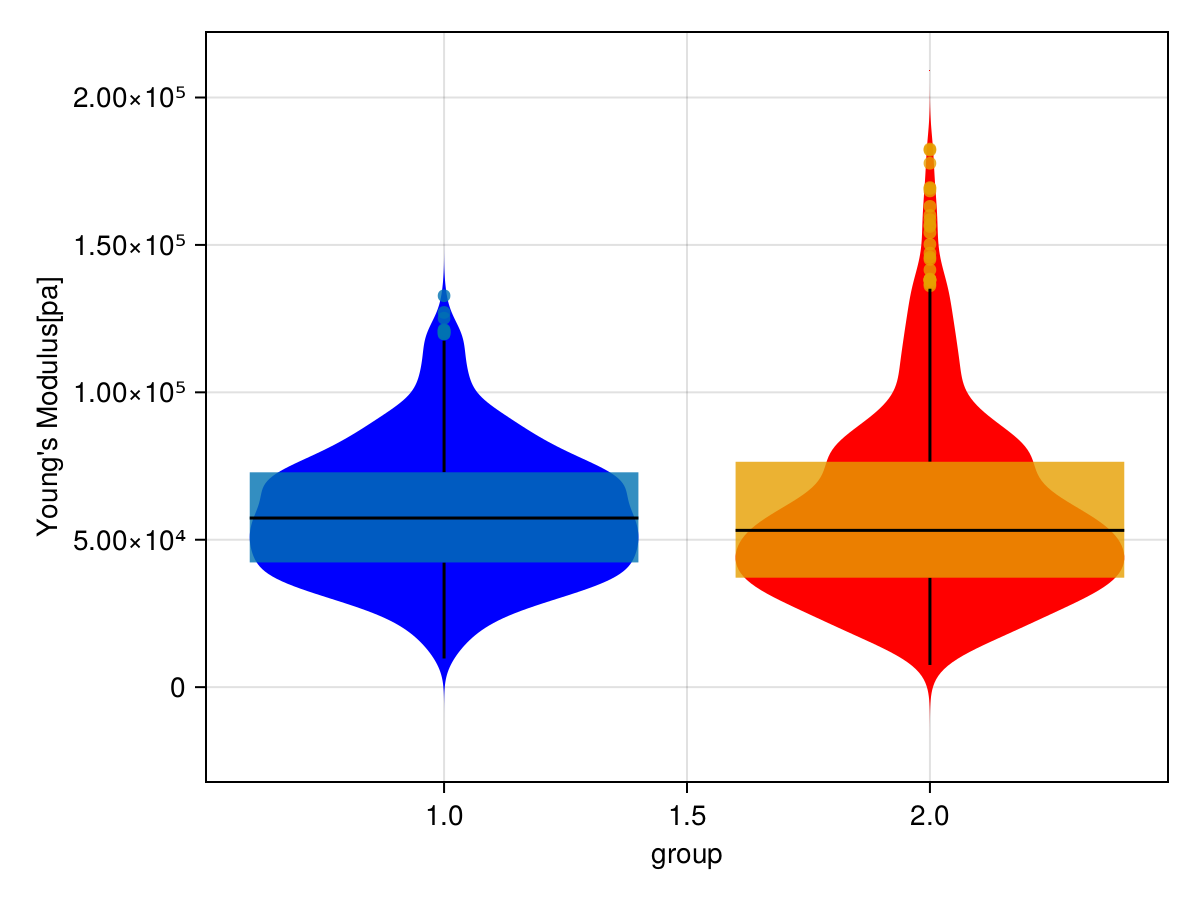
\includegraphics[width=0.8\textwidth]{HistogramsAndViolinplot/violinplot.png}
    \caption{Boxplot with IQR and Violoin Plot with Dstribution, in Red the Cells treated with Cytochalasin D and in Blue the Control Cells}
    \label{fig:ViolinPlot}
\end{figure}

%\begin{tcolorbox}[colback=black!80!white, coltext=white]
%\begin{lstlisting}[language=python, basicstyle=\ttfamily\small]
%Population details:
%    parameter of interest:   Mean difference
%    value under h_0:         0
%    point estimate:          267.884
%    95% confidence interval: (-2467.0, 3003.0)
%
%Test summary:
%    outcome with 95% confidence: fail to reject h_0
%    two-sided p-value:           0.8477
%
%Details:
%    number of observations:   [745,768]
%    t-statistic:              0.19212099420751927
%    degrees of freedom:       1511
%    empirical standard error: 1394.3493895086813
%\end{lstlisting}
%\end{tcolorbox}

%\section{Discussion}
%\label{subsec:discussionHC}

Given the limited experimental design with only one replicate for each cell type (treated vs untreated), applying a t-test for statistical comparison is highly questionable. The fundamental assumption of the t-test is the availability of a sufficiently large sample size to draw meaningful conclusions. In this scenario, the lack of replication undermines the statistical power, making it difficult to establish the credibility of any observed differences. Relying on a single data point introduces significant uncertainty and reduces the reliability of the t-test results. \\

Given the constraint of having only one replicate for each cell type, an alternative statistical test is the Mann-Whitney U test. Unlike the t-test, the Mann-Whitney U test is a non-parametric test that does not rely on assumptions about the underlying distribution.\\

\[U_1 = n_1n_2 + \frac{n_1(n_1 + 1)}{2} - R_1\] 
\\
The Mann–Whitney U test, also known as the Wilcoxon rank-sum test, is a nonparametric method for comparing two independent populations, X and Y, based on randomly selected values from each. The test assesses whether the probability of X being greater than Y is equal to the probability of Y being greater than X. It doesn't rely on assumptions of a specific distribution and is applicable to ordinal data. Under the null hypothesis (H0), the distributions of both populations are considered identical, while the alternative hypothesis (H1) suggests a difference between the distributions.
\\
The t-test results(p-value = 0.8477) indicated a lack of statistical significance, suggesting no substantial difference in mean Young's modulus between untreated and treated cells based on the current data. However, it is important to note that published experimental replicates contradict this finding [5], indicating a potential flaw in the experimental design. However, it is known that fixation with paraformaldehyde induces an increase in cellular rigidity. This underscores the need for a more meticulous approach in remaking the experiment to obtain reliable and conclusive results.
\\
\begin{figure}[H]
    \begin{subfigure}{0.45\textwidth}
        \centering
        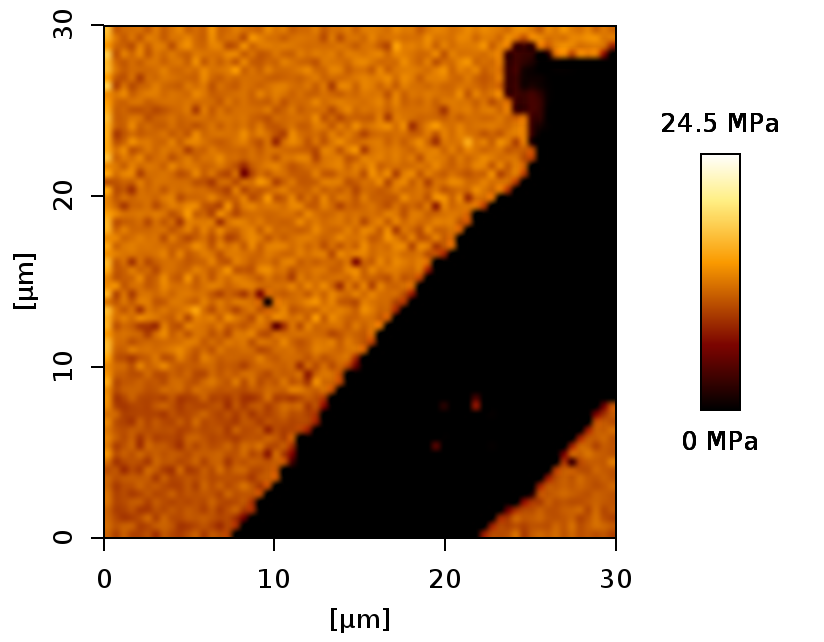
\includegraphics[width=\textwidth]{untreated/modulus.png}
        \caption{Young's Modulus of untreated cells}
        \label{fig:ym_untreated}
    \end{subfigure}
    \begin{subfigure}{0.45\textwidth}
        \centering
        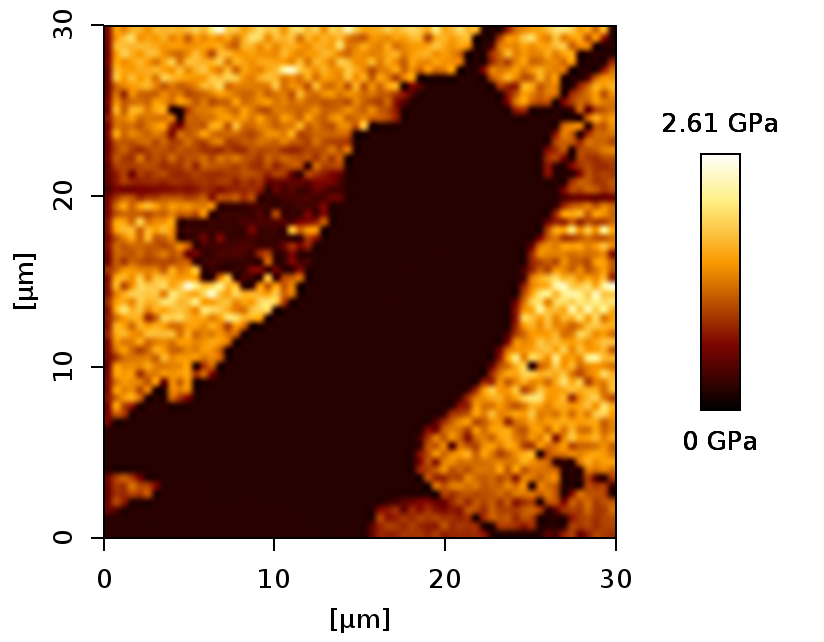
\includegraphics[width=\textwidth]{treated/modulus.png}
        \caption{Young Modulus of treated cells}
        \label{fig:ym_treated}
    \end{subfigure}
    \caption{Young's Modulus Maps of Cells}
    \label{fig:main}
\end{figure}
%\section{Visual Representation of Young's Modulus}
%\label{sec:youngsmodulus}

%Examining a visual representation of Young's modulus is valuable for several reasons. it provides an immediate and intuitive understanding of how materials respond to applied forces. This graphical depiction allows researchers to increase:\newline

%    \textbf{1. Human Interpretability:} Visual representation offers immediate, human-friendly comprehension of material behavior, enhancing interpretation capabilities.
    
%    \textbf{2. Identification of Material Variations:} Visualizing Young's modulus helps pinpoint stiffness variations across materials or within a sample, aiding in understanding heterogeneity.

%    \textbf{3. Artifact Detection:} Visual inspection identifies artifacts or issues not easily discernible through statistical methods, ensuring the reliability of Young's modulus assessment. \newline

%In summary, the visual representation of Young's modulus goes beyond numerical values, offering a human-friendly approach to understanding material behavior and quickly identifying patterns, variations, and potential issues that might be overlooked in a purely statistical analysis.

%\subsection{Results}
%\label{subsec:resultsVR}
Besides, we also acquired the images of the distribution of Young's modulus directly from the JPK program(Figure 5.4). Unfortunately the bar on the right side does not show the correct number. However, these images still indicate the differences on Young's modulus between cells and background. 
The enhancement on the following points may increase the quality of the images.Human interpretability is notably straightforward, as the identification of cell somae becomes immediate.
The aspect of material variation is underscored by the noticeable contrast in color between the cells and the surrounding dish surface, contributing to an instantaneous representation of the softer nature of cells respective to the petri dish in the background.
Furthermore, the enhanced visual representation now allows for the discernment of previously unnoticed striping artifacts in the image on the right, showcasing the comprehensive insights that a graphical depiction of Young's modulus can provide.


%\subsection{Discussion}
%\label{subsec:discussionVR}

%Considering the absence of enough data and time to apply other statistical methods, a quantitative analysis of the images was not possible. Therefore, we will only discuss the two images from a qualitative point of view.\newline

%\textbf{Scale Discrepancy:} The scales on the right side of the images are neither correct nor normalized between the two samples. This misalignment hinders an effective comparison of the mechanical properties of the two samples.

%\textbf{Striping Artifacts:} Striking striping artifacts are evident in the image on the right, potentially skewing measurements and influencing the statistical significance of the results. These artifacts might arise from debris lodged onto the cantilever tip during the experiment.

%\textbf{Inconsistent Background:} The background in the image on the right lacks consistency, raising concerns about potential confounders beyond the Petri Dish Surface. This inconsistency poses a challenge in accounting for all variables in the statistical test.\newline

%Given these qualitative observations, it is imperative to address issues related to scale normalization, striping artifacts, and background consistency to ensure the reliability and robustness of any future quantitative analyses.



%Given the absence of sufficient data and time constraints limiting the application of other statistical methods, a quantitative analysis of the images wasn't feasible. Hence, our focus will be on a qualitative assessment of the two images.

%The images portray scales on their right sides that exhibit inconsistencies between the two samples. This discrepancy in scales impedes an effective comparison of the mechanical properties of the samples.

%Moreover, the image on the right reveals prominent striping artifacts that could potentially distort measurements and significantly affect the statistical validity of the results. These artifacts might have originated from debris sticking onto the cantilever tip during the experimental process.

%Additionally, inconsistencies in the background of the right-side image raise concerns about unaccounted variables beyond the Petri Dish Surface. This lack of uniformity in the background could be caused by Fibroblasts creating Extracellular matrix filaments on the Surface, poseing a further challenge in encompassing all variables within the scope of the statistical test.

%In light of these qualitative observations, it becomes imperative to address issues related to scale normalization, striping artifacts, and background consistency. Doing so will be crucial to ensure the credibility, reliability, and robustness of any future quantitative analyses conducted on these images.
\section{Morphology Differences}
\label{sec:Morphology}

Cell morphology directly influences its function. The cell's shape, determined by its internal structure and cytoskeleton, is adapted to carry out specific tasks. For instance, red blood cells are disc-shaped for efficient oxygen transport, while neurons have elongated structures for signal transmission. Changes in the cytoskeleton, in particular proteins like actin, impact structural integrity and cellular function. [8] \newline
The relationship between shape and function is evident in cellular movement; cells with specific shapes [9], like fibroblasts, are designed for effective migration.\newline
So, considering that the form of a cell is intimately tied to its functionality, alterations in morphology are an optimal characteristic to investigate if we want to compare the effect of Cytochalasin D. 

We anticipate Morphological changes in cells subjected to Cytochalasin D treatment due to the disruption of actin filament synthesis. Actin, a fundamental component of the cytoskeleton, plays a pivotal role in maintaining cell shape, motility, and intracellular transport.\newline

The NIH/3T3 ATCC Fibroblasts serve as an ideal model to observe cytochalasin-induced morphological variations. Through Atomic Force Microscopy (AFM) analysis, we gain morphological insights at the nanoscale by using the Contact Point Height. Giving us a true 3D representation of the Cell .\newline

Finally, by analyzing the morphological disparities from a qualitative point of view, we can confirm that cell function is profoundly disrupted by Cytochalasin D.

%\subsection{Results}
%\label{subsec:resultsMD}

\begin{figure}[H]
    \begin{subfigure}{0.45\textwidth}
        \centering
        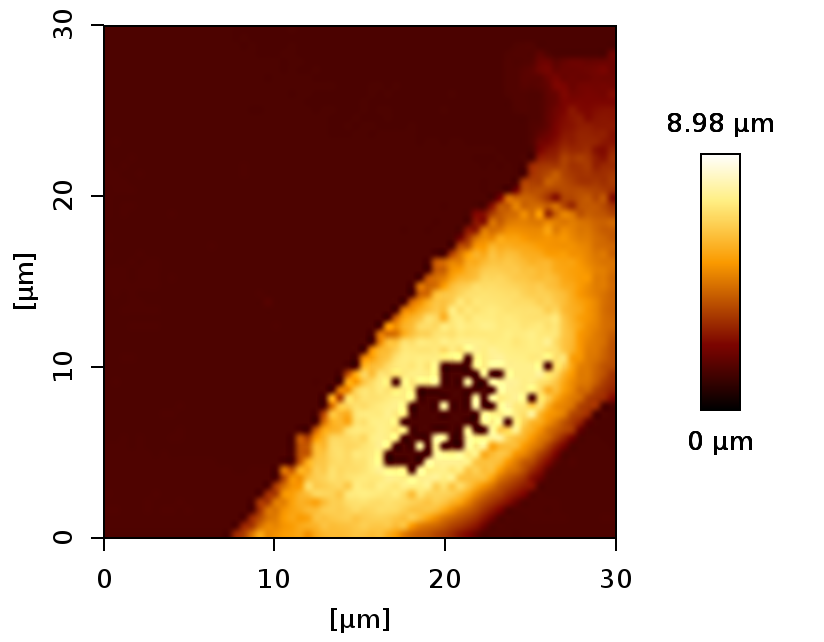
\includegraphics[width=\textwidth]{untreated/image.png}
        \caption{Height Map of untreated cell}
        \label{fig:ym_untreated}
    \end{subfigure}
    \begin{subfigure}{0.45\textwidth}
        \centering
        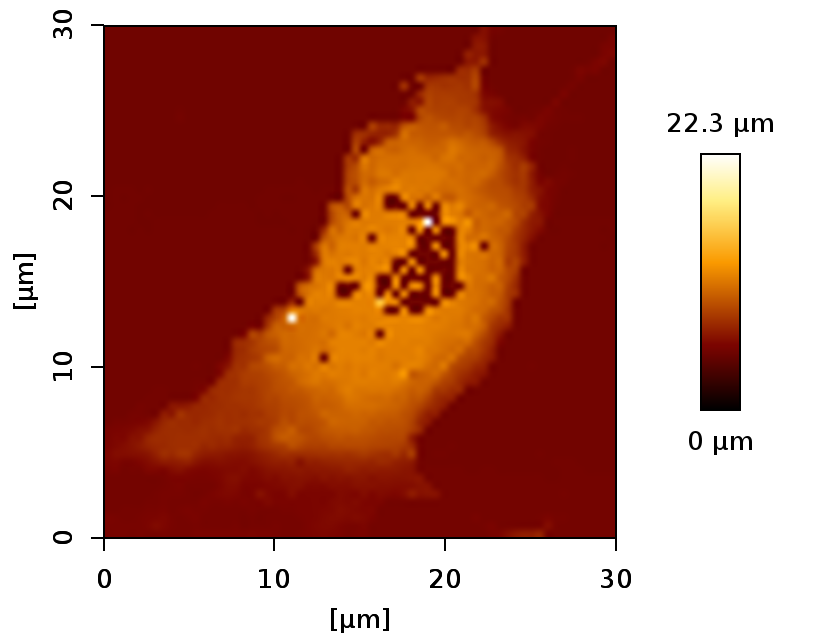
\includegraphics[width=\textwidth]{treated/image.png}
        \caption{Height Map of treated cell}
        \label{fig:ym_treated}
    \end{subfigure}
    \caption{Height Maps of Cells}
    \label{fig:main}
\end{figure}


%\textbf{Missing Data Near Nuclei:}\\
The height maps exhibit missing data near nuclei, a potential artifact from image acquisition or processing. The impact of this missing data on cell morphology analysis and quantitative measurements should be carefully considered. Exploring image processing or reacquisition methods is crucial to minimize or correct these artifacts.\\

%\textbf{Scale Normalization in 3D Views:}\\
The observed flatness in the untreated cell's 3D representation is likely due to scale normalization issues. Proper scale normalization is essential for accurate comparisons between treated and untreated cells in 3D views. Potential corrections for scaling artifacts in 3D representations should be explored.

\begin{figure}[H]
    \begin{subfigure}{0.45\textwidth}
        \centering
        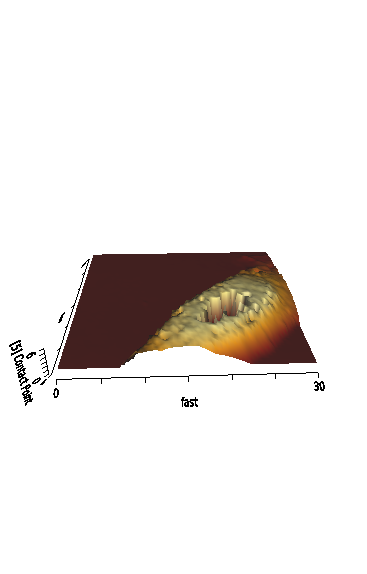
\includegraphics[width=\textwidth]{untreated/map.png}
        \caption{3D View of Height of untreated cell}
        \label{fig:ym_untreated}
    \end{subfigure}
    \begin{subfigure}{0.45\textwidth}
        \centering
        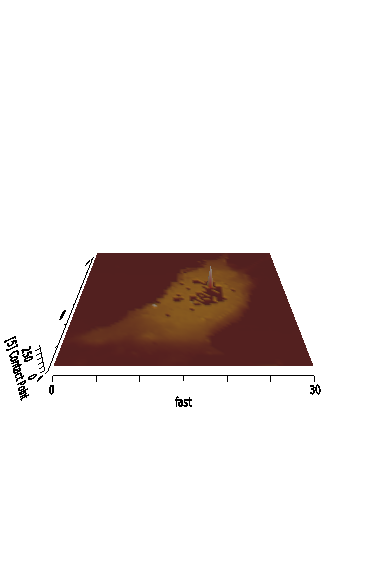
\includegraphics[width=\textwidth]{treated/map.png}
        \caption{3D View of Height of treated cell}
        \label{fig:ym_treated}
    \end{subfigure}
    \caption{Height Maps }
    \label{fig:main}
\end{figure}

%\subsection{Discussion}
%\label{subsec:discussionMD}

%\textbf{Spindle-like Shape in Untreated Cells:}
Untreated cells maintain a spindle-like shape, contrasting with the irregular shapes observed in treated cells.
%\textbf{Filopodia Differences:}
Untreated cells show fewer filopodia, while treated cells exhibit increased filopodia and bulbous structures.
%\textbf{Gradient Uniformity:}
Untreated cells display a more uniform gradient, whereas treated cells appear rougher on the edges with irregular shapes.
%\textbf{Cluster Formation:}
Untreated cells exhibit clusters, contributing to a non-uniform gradient, which is absent in treated cells.
It's crucial to acknowledge potential limitations: we lack multiple images, introducing the possibility of skewed observations due to inexperience with cell shape. These qualitative differences are indicative, and further quantitative analysis is warranted for a comprehensive understanding.
These observations provide valuable insights, but given the constraints and the qualitative nature of the analysis, cautious interpretation is advised.


\chapter{Conclusions}
\label{cha:conclusions}
The study employed Atomic Force Microscopy (AFM) to investigate the impact of cytochalasin D treatment on the mechanical properties of fixed mouse fibroblasts (NIH/3T3 ATCC cell line). The experimental approach involved force-distance measurements using the JPK NW3 AFM in force-volume mode, with the goal of understanding changes in cell stiffness induced by the disruption of actin polymerization.\\

The use of AFM in force-volume mode allowed for the measurement of the mechanical properties of cells, specifically focusing on Young's modulus. Cytochalasin D, a fungal toxin known for its ability to interfere with actin polymerization, served as the treatment agent. The results were analyzed using the Hertz fit model, providing insights into the nanoscale mechanics of the treated cells.\\

We assessed the impact of Cytochalasin D on cell mechanics and morphology, specifically focusing on Young's modulus and cell shape. The null hypothesis ($H_0$) posited no significant difference in Young's modulus between treated and untreated cells, while the alternative hypothesis ($H_1$) suggested a softening effect in treated cells. A t-test was employed for analysis.\\

Results indicated a lack of statistical significance, prompting consideration of the limited experimental design with only one replicate for each cell type. The Mann-Whitney U test was proposed as an alternative, emphasizing the need for replication and a meticulous approach in future experiments.\\

Visual representation of Young's modulus provided immediate interpretability, identifying artifacts not discernible through statistics. Morphology differences highlighted variations in shape, with treated cells exhibiting irregularities. Acknowledging limitations, such as the lack of multiple images, stressed the qualitative nature of the analysis.\\

In conclusion, the study offers insights into Cytochalasin D's effects, but limitations underscore the need for a more robust experimental design. The qualitative observations provide a foundation for further quantitative analysis, emphasizing the complex interplay between cytoskeletal dynamics, mechanical properties, and cell morphology.

\chapter{References}
\label{cha:References}
[1], de Pablo PJ. Introduction to atomic force microscopy. Methods Mol Biol. 2011;783:197-212.

[2], "Mean | Definition, Formula, \& Facts | Britannica". www.britannica.com. 2023-09-22. Retrieved 2023-10-27.

[3],"Median". https://en.wikipedia.org/wiki/Median. 06:03, 16.11.2023

[4], "An introduction to t Test", https://www.scribbr.com/statistics/t-test/, Rebecca Bevans, 31.01.2020

[5], "Mortensen K, Larsson LI. Effects of cytochalasin D on the actin cytoskeleton: association of neoformed actin aggregates with proteins involved in signaling and endocytosis." Cell Mol Life Sci. 2003  doi: 10.1007/s00018-003-3022-x.

[6], "Atomic force microscopy of 3T3 and SW-13 cell lines: an investigation of cell elasticity changes due to fixation.",Codan B, Martinelli V, Mestroni L, Sbaizero O. Mater Sci Eng C Mater Biol Appl. 2013 Aug 1;33(6):3303-8.

[7], "Depth-sensing analysis of cytoskeleton organization based on AFM data".Pogoda, Katarzyna \& Jaczewska, Justyna \& Wiltowska-Zuber, Joanna \& Klymenko, Olesya \& Zuber, Kazimierz \& Fornal, Maria \& Lekka, Malgorzata. (2012).  European biophysics journal : EBJ. 41. 79-87. 10.1007/s00249-011-0761-9. 

[8], " Actin in Action" Marx, V. Actin in action. Nat Methods 20, 178–182 (2023). https://doi.org/10.1038/s41592-022-01762-2

[9], "Restraint of Human Skin Fibroblast Motility, Migration, and Cell Surface Actin Dynamics, by Pannexin 1 and P2X7 Receptor Signaling" Flores-Muñoz C, Maripillán J, Vásquez-Navarrete J, Novoa-Molina J, Ceriani R, Sánchez HA, Abbott AC, Weinstein-Oppenheimer C, Brown DI, Cárdenas AM, García IE, Martínez AD. Restraint of Human Skin Fibroblast Motility, Migration, and Cell Surface Actin Dynamics, by Pannexin 1 and P2X7 Receptor Signaling. Int J Mol Sci. 2021 Jan 22;22(3):1069. doi: 10.3390/ijms22031069. PMID: 33499026; PMCID: PMC7865282.

\end{document}
